\documentclass[border=10pt]{standalone}
\usepackage{tikz}
\usetikzlibrary{calc, shapes.geometric, decorations.pathreplacing}

\begin{document}

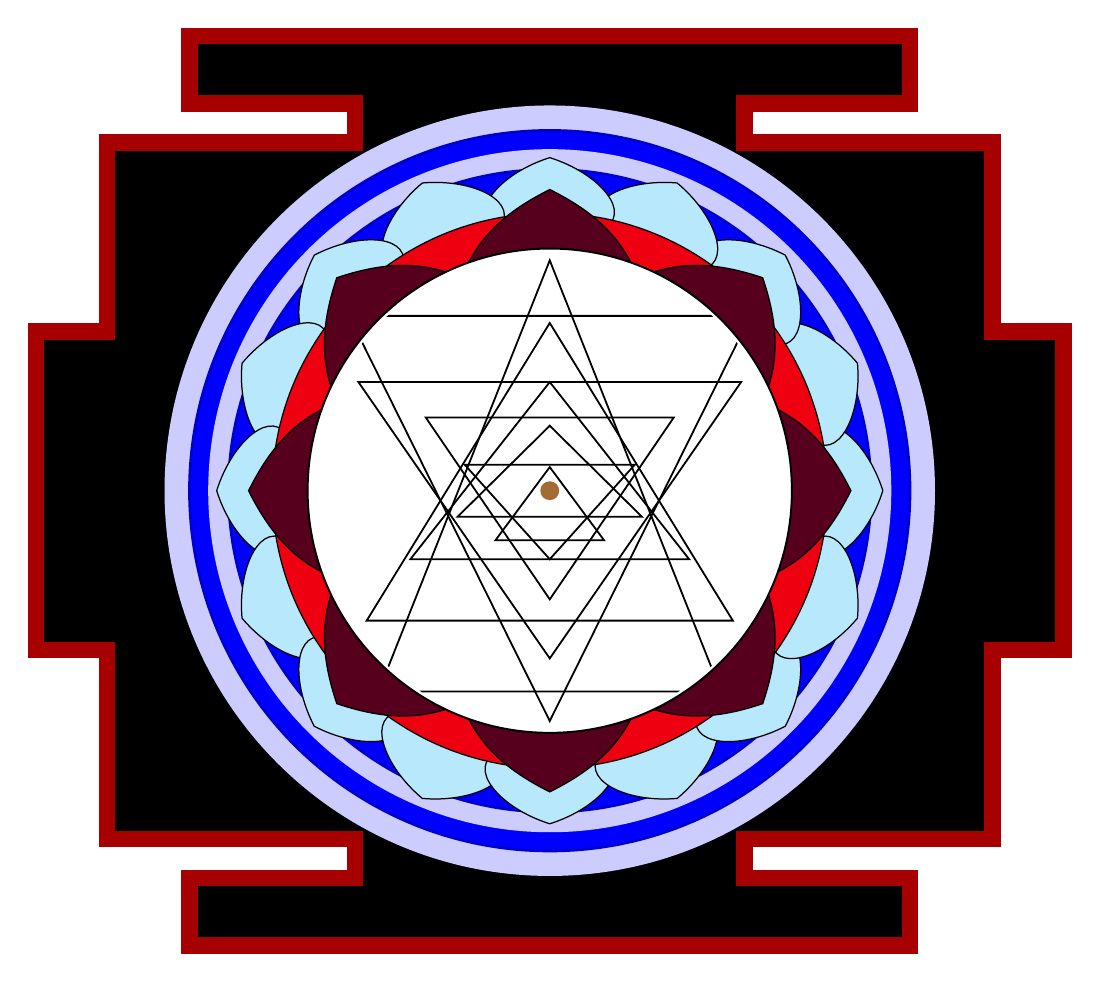
\begin{tikzpicture}[scale=1.5]

% Continuous black temple-like outer frame with a dark red stepped outline
\path[fill=black, draw=red!65!black, line width=6pt, line join=miter]
    (-3.05,3.85) -- (3.05,3.85) -- (3.05,3.28) -- (1.65,3.28) --
    (1.65,2.95) -- (3.75,2.95) -- (3.75,1.35) -- (4.35,1.35) --
    (4.35,-1.35) -- (3.75,-1.35) -- (3.75,-2.95) -- (1.65,-2.95) --
    (1.65,-3.28) -- (3.05,-3.28) -- (3.05,-3.85) -- (-3.05,-3.85) --
    (-3.05,-3.28) -- (-1.65,-3.28) -- (-1.65,-2.95) -- (-3.75,-2.95) --
    (-3.75,-1.35) -- (-4.35,-1.35) -- (-4.35,1.35) -- (-3.75,1.35) --
    (-3.75,2.95) -- (-1.65,2.95) -- (-1.65,3.28) -- (-3.05,3.28) -- cycle;

% Outer circular field and blue ring
\draw[fill=blue!20!white, draw=blue!20!white, line width=1pt] (0,0) circle (3.25);
\draw[fill=blue, draw=blue!80!black, line width=1pt] (0,0) circle (3.05);
\draw[fill=blue!20!white, draw=blue!20!white, line width=1pt] (0,0) circle (2.88);
\draw[fill=blue, draw=blue!80!black, line width=1pt] (0,0) circle (2.72);

% Scalloped cyan lotus petals around the blue ring
\foreach \i in {0,22.5,...,337.5} {
    \path[fill=cyan!28!white, draw=black, line width=0.45pt]
        (\i-11.25:2.25)
        .. controls (\i-17:2.45) and (\i-9:2.72) .. (\i:2.82)
        .. controls (\i+9:2.72) and (\i+17:2.45) .. (\i+11.25:2.25)
        .. controls (\i+4:2.36) and (\i-4:2.36) .. cycle;
}

% Separate magenta and dark-purple petal ring
\draw[fill=red!75!purple, draw=black, line width=0.45pt] (0,0) circle (2.35);
\foreach \i in {0,45,...,315} {
    \path[fill=purple!45!black, draw=black, line width=0.45pt]
        (\i-22.5:1.95)
        .. controls (\i-15:2.28) and (\i-7:2.42) .. (\i:2.55)
        .. controls (\i+7:2.42) and (\i+15:2.28) .. (\i+22.5:1.95)
        .. controls (\i+9:1.72) and (\i-9:1.72) .. cycle;
}

% White central circular disk
\draw[fill=white, draw=black, line width=0.7pt] (0,0) circle (2.05);

% Sri Yantra: nested interlocking upward and downward triangles
\begin{scope}
\clip (0,0) circle (2.02);
\draw[black, line width=0.65pt] (-1.45,-1.70) -- (0,1.95) -- (1.45,-1.70) -- cycle;
\draw[black, line width=0.65pt] (-1.70,1.48) -- (0,-1.95) -- (1.70,1.48) -- cycle;
\draw[black, line width=0.65pt] (-1.55,-1.10) -- (0,1.42) -- (1.55,-1.10) -- cycle;
\draw[black, line width=0.65pt] (-1.62,0.92) -- (0,-1.42) -- (1.62,0.92) -- cycle;
\draw[black, line width=0.65pt] (-1.18,-0.58) -- (0,0.92) -- (1.18,-0.58) -- cycle;
\draw[black, line width=0.65pt] (-1.05,0.62) -- (0,-0.92) -- (1.05,0.62) -- cycle;
\draw[black, line width=0.65pt] (-0.78,-0.22) -- (0,0.55) -- (0.78,-0.22) -- cycle;
\draw[black, line width=0.65pt] (-0.72,0.22) -- (0,-0.58) -- (0.72,0.22) -- cycle;
\draw[black, line width=0.65pt] (-0.46,-0.42) -- (0,0.20) -- (0.46,-0.42) -- cycle;
\end{scope}

% Bindu (brown dot)
\fill[brown!85!black] (0,0) circle (0.08);

\end{tikzpicture}

\end{document}
